\section{Aspect fonctionnelle}
	
	\subsection{Décomposition fonctionnelle}
	
	L'analyse du sujet a conduit à quatre fonctions principales décomposées en sous-fonctions selon le diagramme hiérarchique de la figure \ref{hier} :
	
	\begin{itemize}
		\item Acquérir les informations, 
		\item Traiter les informations,
		\item Afficher les informations,
		\item Communiquer
	\end{itemize}

L'analyse du modèle a mis en évidence, s'il était besoin, le rôle crucial
de la communication entre contrôleur et pilote dans la fourniture du service de contrôle, d'alerte et de surveillance. Sur le plan métier, la radio comme moyen de communication constitue le maillon faible des systèmes ATC actuel. En ce sens, la modélisation permet 
de mettre en évidence des failles du domaine réel ce qui constitue une source de progrès. 
	
	\begin{figure}[H]
		\begin{center}	
			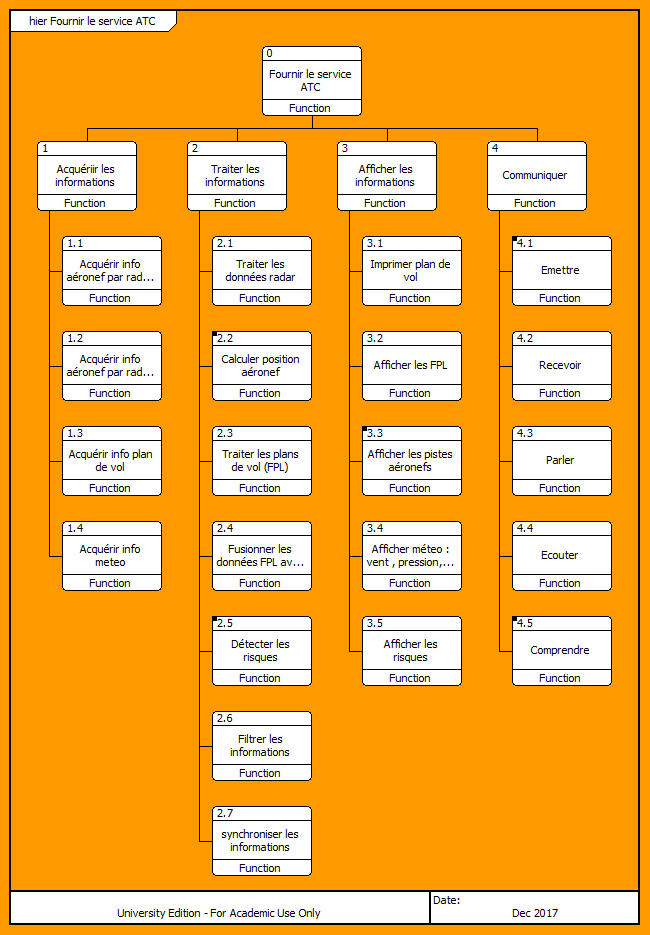
\includegraphics[scale=0.85]{images/hierarchique}
			\caption{Diagramme hiérarchique des fonctions}
			\label{hier}
		\end{center}
	\end{figure}
	
	\subsection{Scénario fonctionnel}

    Les diagrammes d'activités, EFFBD ou de séquence permettent de capturer un ou plusieurs scenarii du système modélisé. La démarche utilisée a consisté à créé un diagramme EFFBD dans CORE en utilisant uniquement les fonctions feuille puis de travailler sur le diagramme N2 pour l'ajout des items. Un exemple est donné en figure \ref{atc}. Le scénario associé à l'ensemble des fonctions feuille se trouve à l'adresse  \url{https://github.com/kad15/AF/blob/master/LIVRABLES_ATC_YUAN_BELDJILALI/question%207%20%20scenario%20fonctionnel%20unique.png}
    
    	\begin{figure}[H]
    	\begin{center}	
    		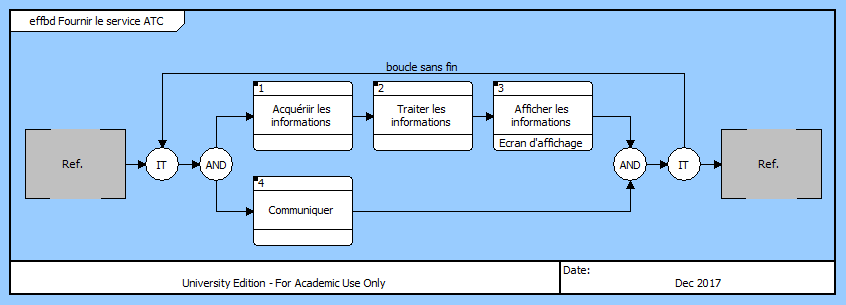
\includegraphics[scale=0.75]{images/atc}
    		\caption{Diagramme EFFBD simplifié du service ATC}
    		\label{atc}
    	\end{center}
    \end{figure}
    